\begin{homeworkProblem}[18]
Recall the denotation in this problem:
\[
    \begin{aligned}
        p &= \text{frequency of allele }A \\
        q &= \text{frequency of allele }a \\
        u &= \text{frequency of }AA\text{ genotype} \\
        v &= \text{frequency of }Aa\text{ genotype}  \\
        w &= \text{frequency of }aa\text{ genotype}  \\
    \end{aligned}
\]
\begin{enumerate}
\item From the definition of $u$, $v$ and $w$, it's clear that $u +v + w = 1$.
The frequency of allele $A = u + \frac{1}{2}v$ and the frequency of allele $a
= \frac{1}{2}v + w$. It's easy to see that $p + q = u + \frac{1}{2}v + \frac{1}{2}
v + w = 1$.
\item Table 3.1 is filled up and presented below as Table 1.
The new values are marked in red.
\begin{table}[h!]
\centering
\begin{tabular}{|c|c|c|c|c|c|}
\hline
\multirow{3}{*}{ } &
\multirow{3}{*}{Genotype} &
\multirow{3}{*}{Frequency \%} &
\multicolumn{3}{|c|}{Fathers}\\
\cline{4-6}
& & & $AA$ & $Aa$ & $aa$ \\ \cline{4-6}
& & & $u$ & $v$ & $w$ \\
\hline
\multirow{3}{*}{Mothers} & $AA$ & $u$ & $u^2$ & $uv$ & $uw$\\
& $Aa$ & $v$ & {\color{red} $uv$} & $v^2$ & {\color{red} $vw$}\\
& $aa$ & $w$ & {\color{red} $uw$} & {\color{red}$vw$} & {\color{red}$w^2$} \\
\hline
\end{tabular}
\end{table}

\item The figure is shown as below.
\begin{figure}[h]
    \centering
    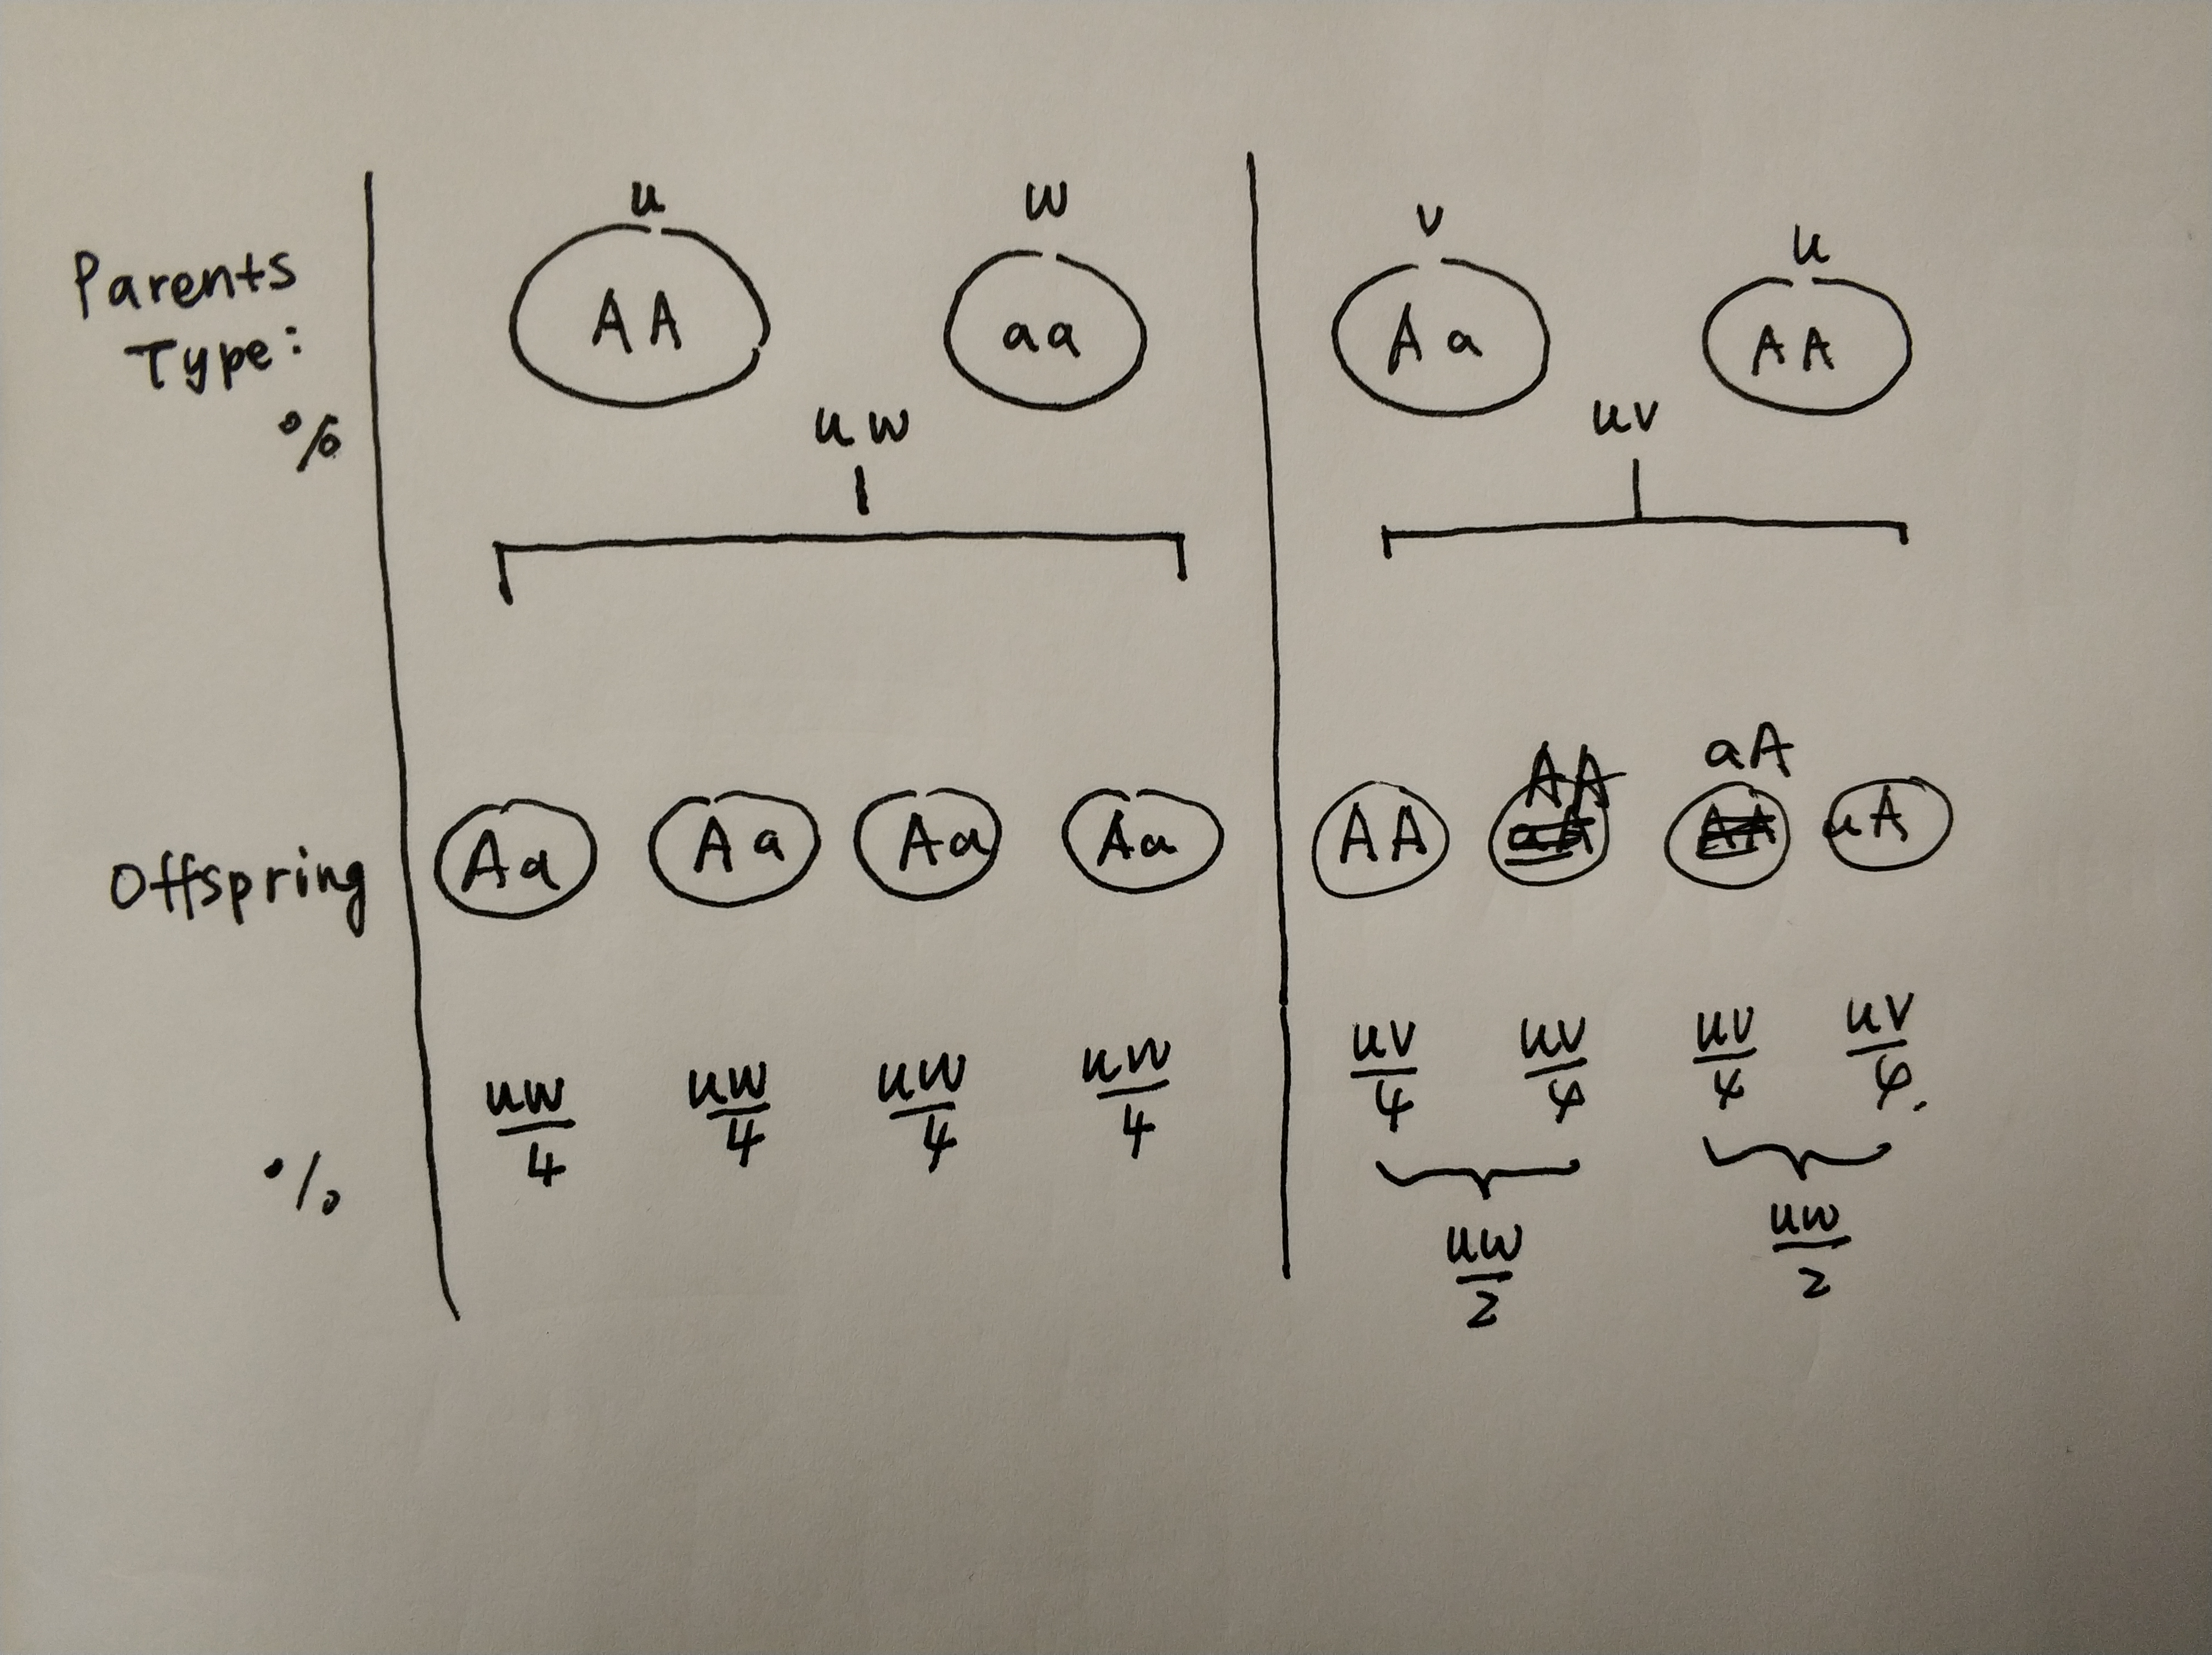
\includegraphics[width=0.5\linewidth]{fig/fig1.jpg}
\end{figure}

\item Table 3.2 is filled up and presented below as Table 2.
The new values are marked in red.

\begin{table}[h!]
    \centering
    \begin{tabular}{|c|c|c|c|c|}
    \hline
    \multirow{2}{*}{Type of Parents} & \multirow{2}{*}{Genotype} &
    \multicolumn{3}{|c|}{Offspring Genotype Frequencies}\\
    \cline{3-5}
                    &             & $AA$    & $Aa$        & $aa$       \\\hline
    $AA \times AA$  & $u^2$       & $u^2$   & $0$         & $0$        \\
    $AA \times Aa$  & $2uv$       & $uv$    & $uv$        & $0$        \\
    $AA \times aa$  & \red{$2uw$} & $0$     & \red{$2uw$} & \red{$0$}  \\
    $Aa \times Aa$  & $v^2$       & $v^2/4$ & $v^2/2$     & $v^2/4$    \\
    $Aa \times aa$  & \red{$2vw$} & $0$     & \red{$vw$}  & \red{$vw$} \\
    $aa \times aa$  & \red{$w^2$} & $0$     & \red{$0$}   & \red{$w^2$}\\\cline{3-5}
                    & Total
                    & $(u^2 + uv + v^2/4)$
                    & \red{$(uv + 2uw + vw + v^2/2)$}
                    &\red{$(w^2 + vw + v^2/4)$}\\
    \hline
    \end{tabular}
\end{table}

\pagebreak
\item It can be seen clearly in the table above that the frequencies are
governed by \begin{align}
    u_{n+1} &= u_n^2 + u_nv_n + \frac{1}{4}v_n^2, \label{eq:u}\\
    v_{n+1} &= u_nv_n + 2u_nw_n + \frac{1}{2}v_n^2 + v_nw_n,\label{eq:v}\\
    w_{n+1} &= \frac{1}{4}v_n^2 + v_nw_n + w_n^2.
\end{align}
% Problem (f)
\item \[
\begin{aligned}
    u_{n+1} + v_{n+1} + w_{n+1} &=
    (u_n^2 + u_nv_n + \frac{1}{4}v_n^2) + (u_nv_n + 2u_nw_n + \frac{1}{2}v_n^2 +
    v_nw_n) + (\frac{1}{4}v_n^2 + v_nw_n + w_n^2)\\
    &= u_n^2 + 2u_nv_n + v_n^2 + 2v_nw_n + 2u_nw_n + w_n^2\\
    &= (u_n+v_n)^2 + 2(u_n+v_n)w_n + w_n^2\\
    &= (u_n+v_n+w_n)^2
\end{aligned}
\]
According to the original setting we know that $u_n + v_n + w_n = 1$. Henceforth,
we've proven that $u_{n+1} + v_{n+1} + w_{n+1} = 1$.

% Problem (g)
\item At steady states $\left(\bar u, \bar v, \bar w\right)$, we have
\begin{align}
    \bar u &= \bar u^2 + \bar u \bar v + \frac{1}{4} \bar v^2, \label{eq:u_steady}\\
    \bar v &= \bar u \bar v + 2\bar u \bar w + \frac{1}{2}\bar v^2 + \bar v \bar w,\\
    \bar w &= \frac{1}{4} \bar v^2 + \bar v \bar w + \bar w^2.
\end{align}
Divided $\bar u$ on both sides of \eqref{eq:u_steady} (since $\bar u$ is not
very likely if not impossible to be $0$ this is doable), we can get \[
    1 = \bar u + \bar v + \frac{\bar v^2}{\bar u}
\]
From (f) we know that $\bar u + \bar v + \bar w = 1$, so \[
    \begin{aligned}
        \bar u + \bar v + \bar w &= \bar u + \bar v + \frac{\bar v^2}{\bar u}\\
        \bar w &= \frac{\bar v^2}{\bar u}\\
        \bar u &= \bar{v}^2 / \bar{w}
    \end{aligned}
\] \qed
% Problem (h)
\item From (f) we know that $w_{n+1} = 1 - u_{n+1} - v_{n+1}$. It can also be
written as $w_n = 1 - u_n - v_n$. Substituting this back into \eqref{eq:u} and
\eqref{eq:v} gives:\begin{equation}
    u_{n+1} = u_n^2 + u_nv_n + \frac{1}{4}v_n^2, \label{eq:u_reduce}
\end{equation}
\begin{equation}
    \begin{split}
    v_{n+1} &= u_nv_n + 2u_n(1 - u_n - v_n) + \frac{1}{2}v_n^2 +
    v_n(1 - u_n - v_n)\\
    &= -2u_n^2 -2u_nv_n-\frac{v_n^2}{2}+v_n+2u_n\label{eq:v_reduce}
    \end{split}
\end{equation}

% Problem (i)
\item From \eqref{eq:u_reduce} it's trivial to see that
\[
    u_{n+1} = \left(u_n + \frac{v_n}{2}\right)^2
\]
And we have \[
    \begin{aligned}
        v_{n+1} &= (u_n + \frac{1}{2}v_{n})[2 - 2 (u_n + \frac{1}{2}v_n)]\\
        &= 2u_n + v_n - 2(u_n + \frac{1}{2}v_n)^2\\
        &= 2u_n + v_n - 2u_n^2 - 2u_nv_n - \frac{v_n^2}{2},
    \end{aligned}
\]which is exactly \eqref{eq:v_reduce}.

% Problem (j)
\item Let $X$ represents $u_n + \frac{v_n}{2}$, then:\[
\begin{aligned}
    u_{n+1} + \frac{v_{n+1}}{2}
    &= X^2 + X(1 - X)\\
    &= X
\end{aligned}\\
\quad i.e.,
\left(u_{n+1} + \frac{v_{n+1}}{2}\right) =
\left(u_n + \frac{v_n}{2}\right)
\]

% Problem (k)
\item Recall that \[
    \begin{aligned}
        p_n &= u_n + \frac{v_n}{2}\\
        q_n &= \frac{v_n}{2} + w_n
    \end{aligned}
\]
So, \[
    \begin{aligned}
        p_{n+1} &= u_{n+1} + \frac{v_{n+1}}{2}\\
        q_{n+1} &= \frac{v_{n+1}}{2} + w_{n+1}
    \end{aligned}
\]
We've known from (j) that \[
    \left(u_{n+1} + \frac{v_{n+1}}{2}\right) = \left(u_n + \frac{v_n}{2}\right)
\]
which means $p_{n+1} = p_n$.
From (a) we know that $p + q = 1$. Since $p$ doesn't change accross generations,
$q$ also trivially won't change. 
I don't understand why we need to use $p^2 + 2pq + q^2 = 1$ to prove this.
\end{enumerate}
\end{homeworkProblem}